Una vez corroborado que el error ya no ocurrió nuevamente, se procedió a ingresar la señal del lazo de corriente para controlar el variador de velocidad.

Para la comunicación del \textbf{Arduino} con el variador de velocidad se decidió utilizar un lazo de corriente de 0-20mA, este tiene ventajas sobre el lazo de tensión ya que el utilizado es más estable en largas distancias y más inmune a los ruidos eléctricos e interferencias electromagnéticas respecto al lazo de tensión. Normalmente, se utilizan lazos de corriente de 4-20mA para poder observar si hubiera fallas en el circuito, pero este modelo de variador, tiene el piso del lazo de corriente en 0mA, el cual fue modificado para que sea utilizado de 4 a 20mA. Cabe mencionar, que el variador podía ser controlado por cualquiera de los dos métodos de lazos.

A continuación se observará la placa interna del variador con sus respectivas borneras por donde ingresará la señal de corriente del lazo de control y el jummper que se tuvo en cuenta para que sea lazo de corriente y no de tensión.

\begin{figure}[htbp]
	\centering
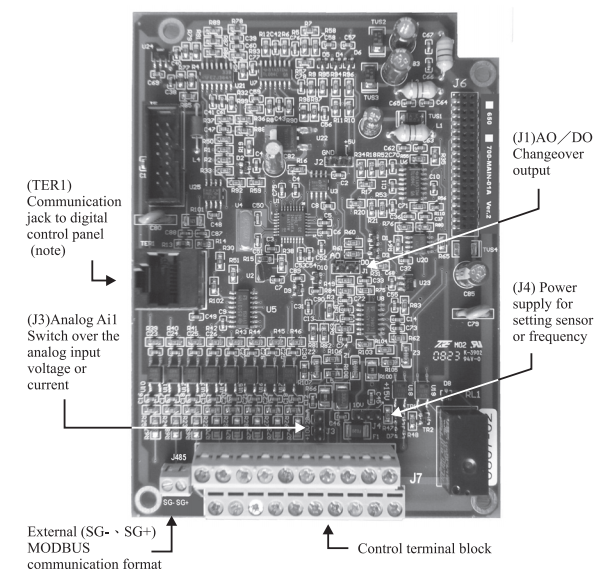
\includegraphics[width=0.7\linewidth]{imagenes/placa_ls}
\caption{Placa de control}
\label{fig:placals}
\end{figure}


\begin{figure}[h]
	\centering
	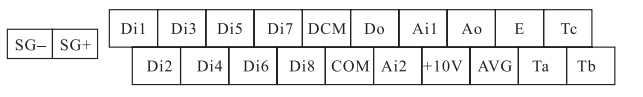
\includegraphics[width=0.7\linewidth]{imagenes/terminales.png}
	\caption{Terminales de control}
	\label{fig:born}
\end{figure}

La señal para controlar el variador de velocidad fue generada por una señal PWM estipulada a través de la librería TIMEROne. La instrucción Timer1.inizialize(period)
 de Arduino inicializa el timer con el valor de period, este valor es el tiempo en el que se dispara el temporizador y en el caso de este proyecto es de 40 microsegundos.
 
El otro comando que se utilizó fue Timer1.pwm(pin, duty) que establece el número de pin, en este caso pin 9 y “duty” es un valor entre 0 y 1023 establecido por la programación. 
Esta señal de salida, fue necesario transformarla al lazo de corriente utilizado para establecer la señal al variador de velocidad. Esto se realizó a través de una placa adaptadora con un filtro generada por nosotros.
\begin{figure}[htbp]
	\centering
	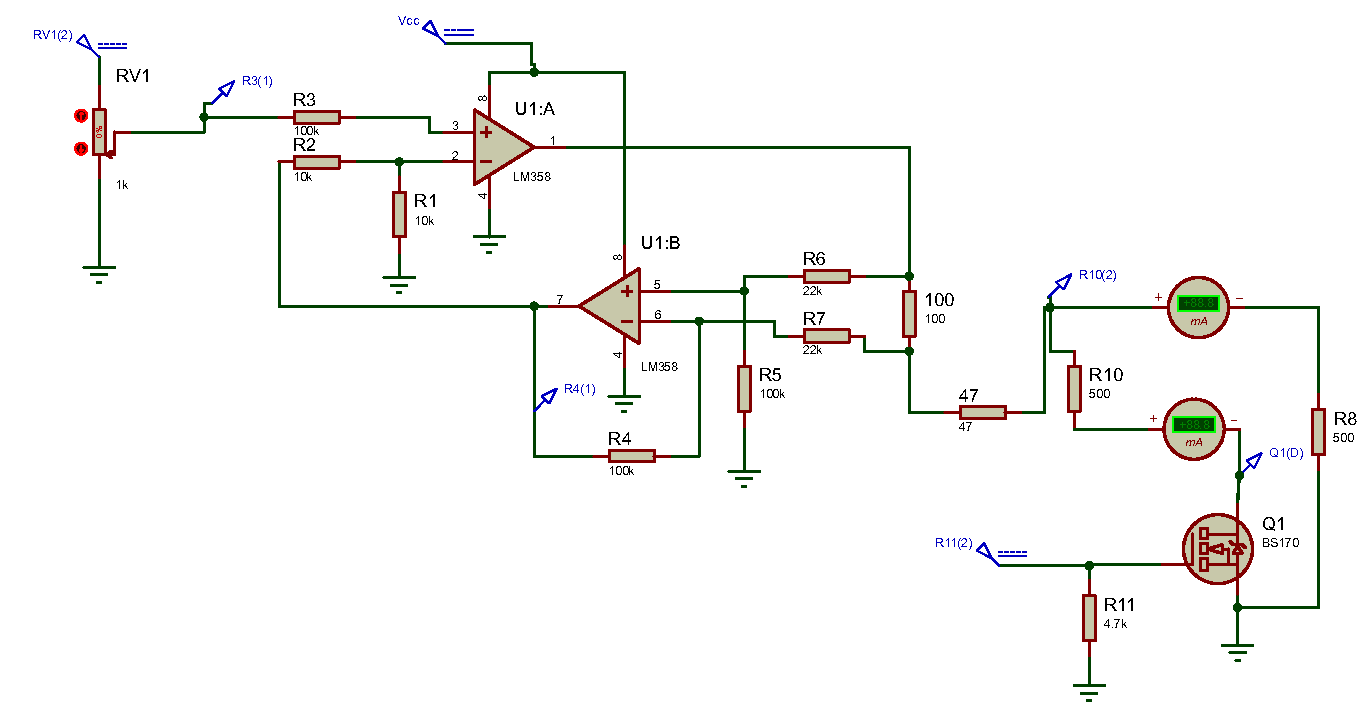
\includegraphics[width=0.8\linewidth]{imagenes/plano_DC.pdf}
	\caption{Placa adaptadora de señal}
	\label{fig:adapt}
\end{figure}

\subsection{Captura de datos por puerto serie}
\begin{tcolorbox}[colback=blue!5!white,colframe=blue!75!black,title=Processing]
    Es un lenguaje de programación basado en Java, aunque hace uso de una sintaxis simplificada y de un modelo de programación de gráficos.
    \end{tcolorbox}
Para capturar los datos, primeramente se utilizó Matlab, como se necesitó visualizar los valores en tiempo real y luego guardar la tabla con vectores, este programa producía errores en la capturación de datos.
Para solucionar el inconveniente anteriormente nombrado, se utilizó un código generado en Processing. Con este código, se capturó los valores, se observaba el valor numérico estimado de la velocidad y se lograba ingresar el valor del escalón requerido para tomar la planta. (Figura \ref{fig:Proce})

\begin{center}
    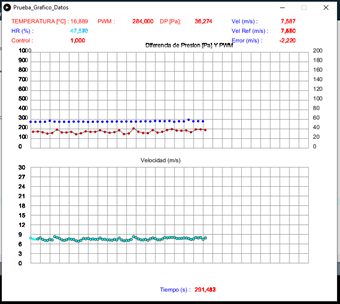
\includegraphics[scale=0.7]{serial_proc.png}
    \captionof{figure}{Pantalla Processing}
    \label{fig:Proce}    
\end{center}

\subsection{Estimación de la planta}
    \subsubsection{Diagrama de trabajo}

Para realizar la estimación de la planta se genera un diagrama de bloques del procedimiento que se siguió de forma resumida.

\begin{figure}[htb]
	\centering
	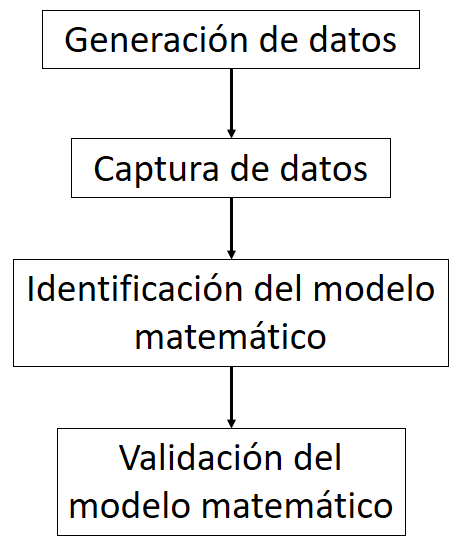
\includegraphics[scale=0.4]{planta_d.png}
	\captionof{figure}{Diagrama de bloques del procedimiento de modelado de la planta}
	\label{fig:planta_d}
\end{figure}

 \textbf{Generación de datos:}  se hizo diversas pruebas para obtener la mayor cantidad de información en la respuesta.

 \textbf{Captura de datos:} A través del puerto serie y con Processing se realiza el almacenamiento de los datos de respuesta del sistema ante el estímulo de las señales de excitación. Posteriormente, el análisis de los datos y la generación de las gráficas correspondientes es realizado por medio de rutinas de código implementadas en Matlab.

 \textbf{Identificación del modelo matemático:} Se utilizaron varios métodos numéricos para la estimación.

 \textbf{Validación del modelo matemático:} una vez obtenida la mejor estimación, se efectuó una validación adicional a partir de la comparación de datos experimentales con los teóricos generados por escalones.






    \subsubsection{Método de estimación}

    Una vez que se determinó valores de ventana de filtro, velocidad de conmutación de PWM, tiempos de aceleración y desaceleración, etc. Se utilizó el modo de ingreso de señal por lazo de corriente en el variador de velocidad. 
    
    La Figura \ref{fig:bloques} muestra un diagrama resumido de los pasos a realizar para tomar datos de la planta. Siendo G(s) el conjunto del túnel de viento, variador de velocidad y motor.
 
    \begin{center}
    	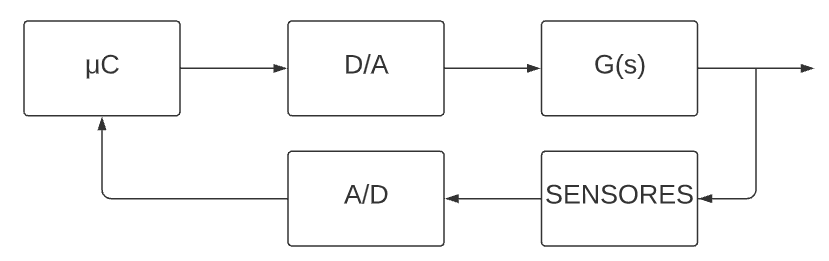
\includegraphics[scale=0.35]{bloques.png}
    	\captionof{figure}{Diagrama en bloques}
    	\label{fig:bloques}    
    \end{center}
    
    Para realizar la estimación de la planta se obtuvo y guardó tablas de datos con Processing, generando por la interfaz distintos escalones de entrada para obtener varias mediciones. En la figura \ref{fig:est2} se observan los datos de dos columnas de las tablas anteriormente generadas.
    
    \begin{figure}[htb]
    	\centering
    	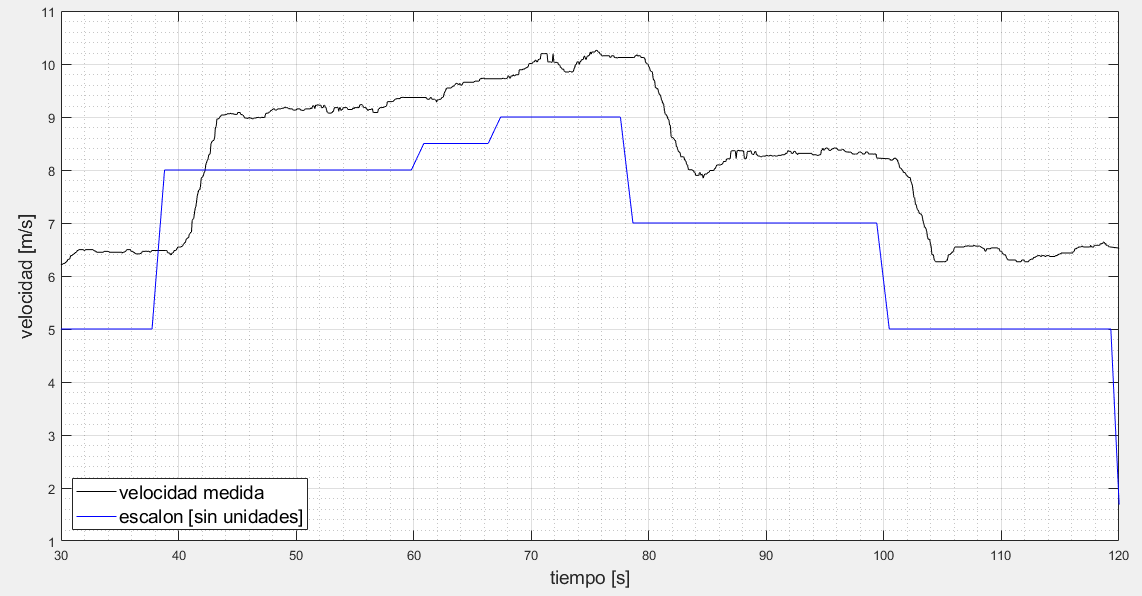
\includegraphics[scale=0.5]{estima.png} %pruba_1 del 0607
    	\captionof{figure}{Mediciones de velocidad a partir de distintos escalones dados}
    	\label{fig:est2}    
    \end{figure}
    
    Seguidamente, se procedió a generar un nuevo código de Matlab donde se cargaron los valores obtenidos de la figura (a) \ref{fig:pl2} para realizar la estimación de la planta a través del método \textit{"Strejc"} \cite{pomares2011sistemas}.
    
    \begin{figure}[htbp]
    	\centering
    	\subfigure[Parámetros Strejc]{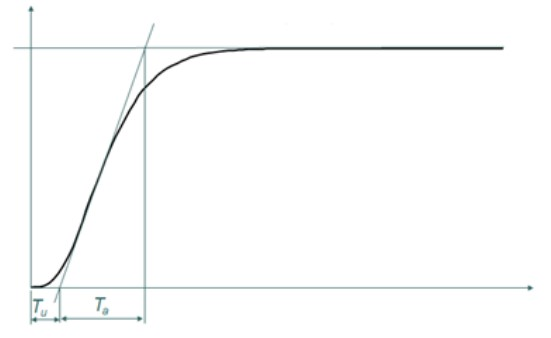
\includegraphics[width=70mm]{parametros.jpg}}
    	\subfigure[Estimación de parámetros]{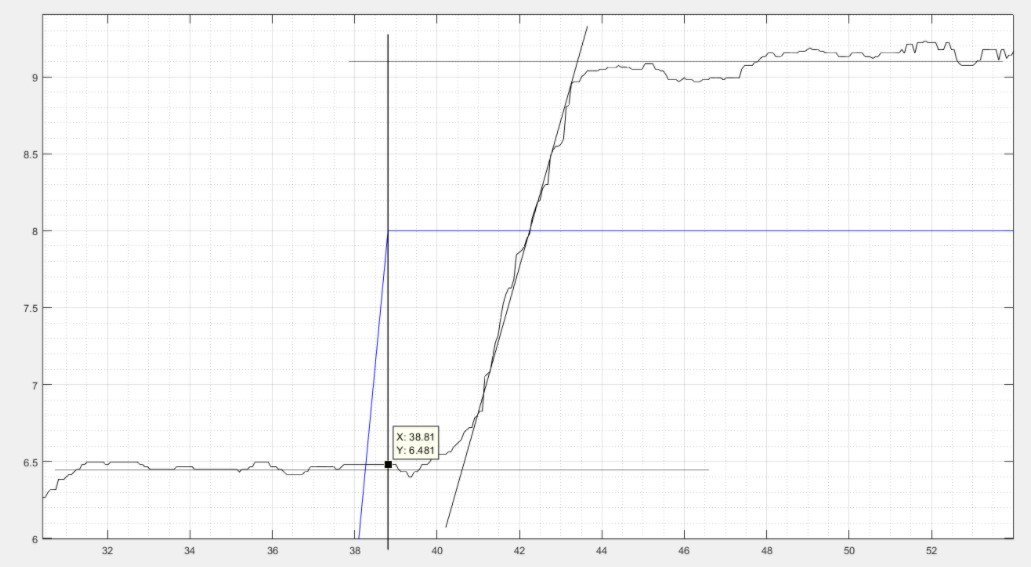
\includegraphics[width=80mm]{planta_est1.jpg}} 
    	\caption{Estimación de planta} \label{fig:pl2}
    \end{figure}
    
    Con ayuda del código y ajustes manuales se llegó a una función de transferencia de segundo orden:
    
    \begin{equation}
    	\frac{Y(s)}{U(s)}=\frac{0,02483}{s^2+1,846s+1,535}
    \end{equation}
    
    Para corroborar la elección de la planta se genreó un archivo en \textit{Simulink} generando como entrada esclaones que se colocaron en el sistema. Luego, el otro código de matlab obtenía estos valores y realizaba la comparación de lo estimado con los valores reales obtenidos en diversas mediciones (Figura \ref{fig:estim2} y Figura \ref{fig:estim3}).
    
    \begin{figure}[htb]
    	\centering
    	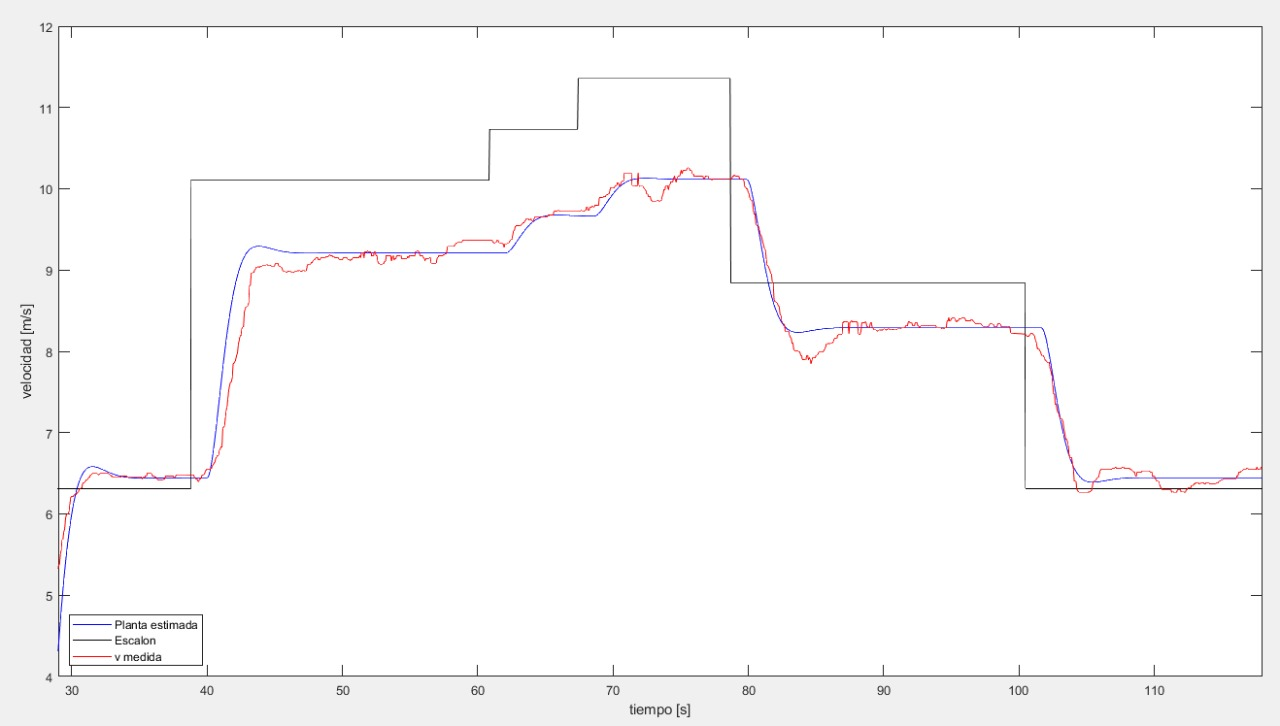
\includegraphics[scale=0.35]{estim2.jpeg}
    	\captionof{figure}{Corroboración de estimación de la planta. Ejemplo 1}
    	\label{fig:estim2}
    \end{figure}

\begin{figure}[htb]
	\centering
	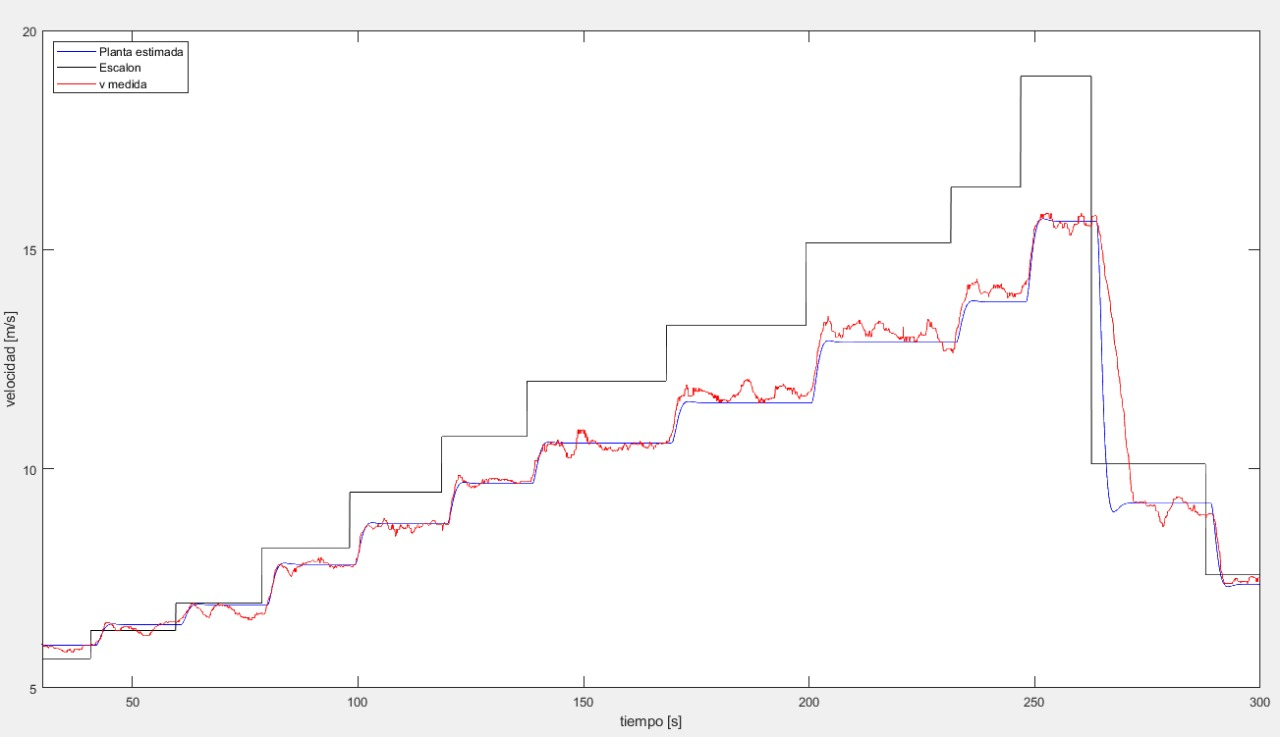
\includegraphics[scale=0.35]{estim3.jpeg}
	\captionof{figure}{Corroboración de estimación de la planta. Ejemplo 2}
	\label{fig:estim3}
\end{figure}
    
       
    \subsection{Control}
    Para relizar una primera estimación de un PID se utilizó la herramienta de \textit{Matlab}, a partir de ahí se realizaban pequeñas modificaciones y se realizaban las simulaciones quedando todos del formato PI (proporcional - integrador).
    Con los valores anteriormente nombrados se realizaron pruebas en el Túnel del viento con escalones de velocidad de referencia de 6 - 7,5 - 8,5 - 7,5 - 7 - 6 m/s, haciendo un total de 5 pruebas, con PI distintos para los mismos escalones. 
    
    \begin{figure}[htb]
    	\centering
    	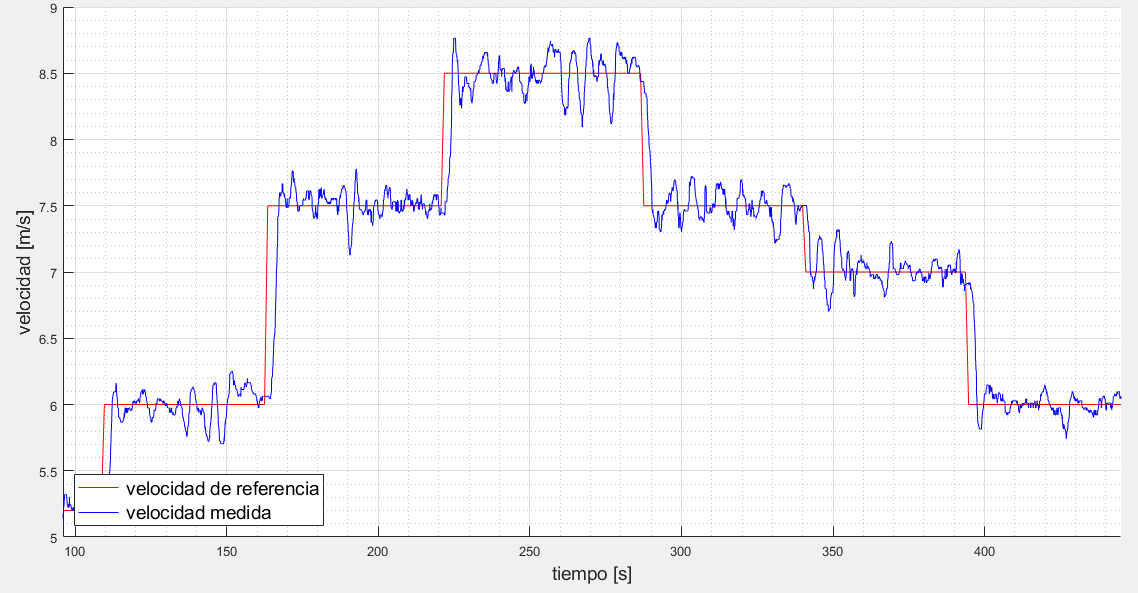
\includegraphics[scale=0.5]{pruebapid.png}
    	\captionof{figure}{Ejemplo de prueba realizada}
    	\label{fig:PI3}
    \end{figure}
    
    Los valores de cada PI utilizados se muestra en la tabla siguiente
    \begin{table}[h]
    	\centering
    	\begin{tabular}{r|r|r|r|r|r|r|}
    		\cline{2-7}
    		\multicolumn{1}{l|}{} & \multicolumn{1}{c|}{\textbf{PI anterior}} & \multicolumn{1}{c|}{\textbf{Prueba3}} & \multicolumn{1}{c|}{\textbf{Prueba4}} & \multicolumn{1}{c|}{\textbf{Prueba5}} & \multicolumn{1}{c|}{\textbf{Prueba6}} & \multicolumn{1}{c|}{\textbf{Prueba7}} \\ \hline
    		\multicolumn{1}{|r|}{\textbf{P=}} & 0.225 & 0.0699 & 0.244 & 0.5451 & 0.6846 & 0.3286 \\ \hline
    		\multicolumn{1}{|r|}{\textbf{I=}} & 0.326 & 0.2035 & 0.2756 & 0.3599 & 0.4183 & 0.3107 \\ \hline
    	\end{tabular}
    \caption{Valores de PID's}
    \end{table}
    
    Uniendo todos los resusltados obtenidos por los distintos PI utilizados se puede realizar las comparaciones para un escalon donde la velocidad sube (figura \ref{fig:pisubuda}) y otro donde la velocidad baja (figura \ref{fig:pibajada}).
    
    \begin{figure}[h!]
    	\centering
    	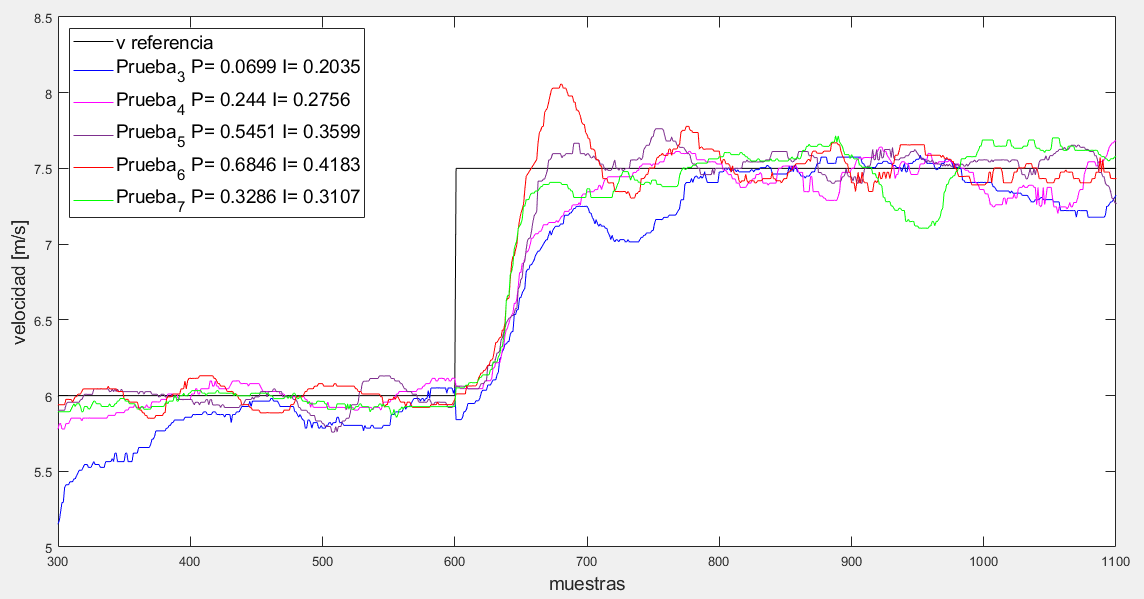
\includegraphics[scale=0.5]{pisubida.png}
    	\captionof{figure}{Comparación de PI, escalon de subida}
    	\label{fig:pisubuda}
    \end{figure}
    
    \begin{figure}[h!]
    	\centering
    	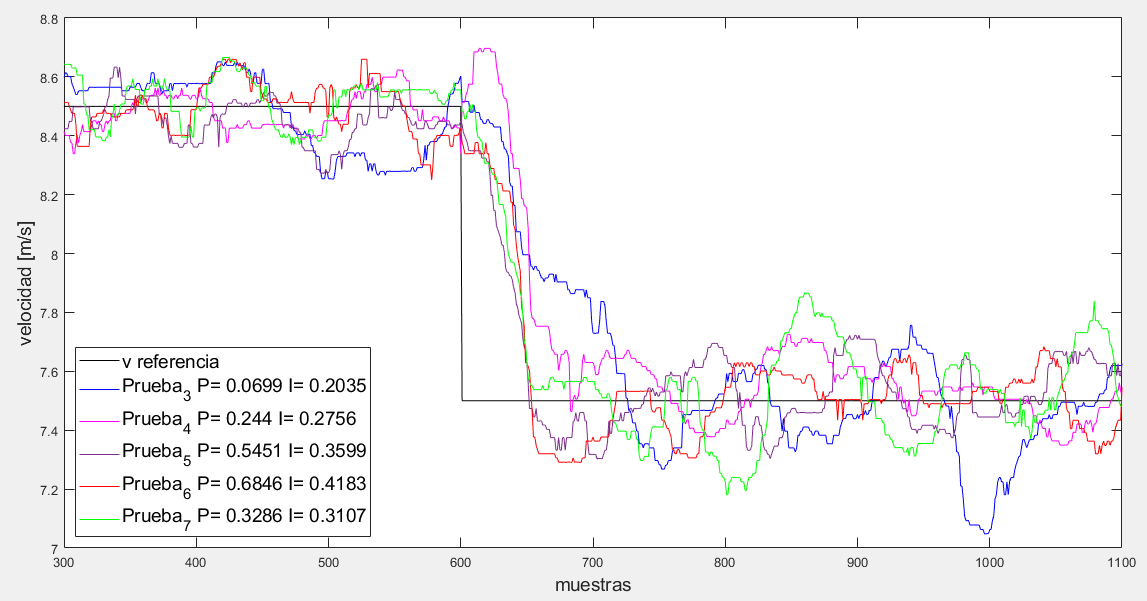
\includegraphics[scale=0.5]{pibajada.png}
    	\captionof{figure}{Comparación de PI, escalon de bajada}
    	\label{fig:pibajada}
    \end{figure}
    
    
    En la figura \ref{fig:mix} se pueden observar el sistema que genera mayor sobrepico, un sistema con una respuesta mas lenta, y un sistema con respuesta intermedia. 
    \begin{figure}[h!]
    	\centering
    	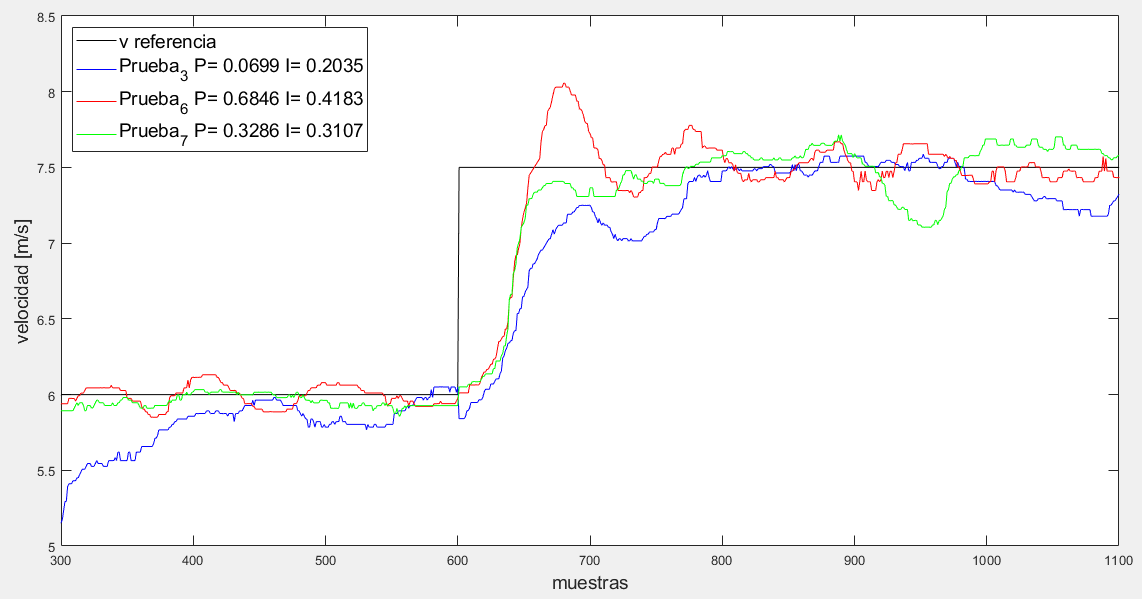
\includegraphics[scale=0.5]{mix.png}
    	\captionof{figure}{Comparación 3 sistemas PI}
    	\label{fig:mix}
    \end{figure}
    
    \newpage